\documentclass[a4paper,
               headsepline,footsepline,
               openany,oneside,chapterprefix,
               12pt]
{scrartcl}
\usepackage{graphicx}
\usepackage{wrapfig} % Required for wrapfigure environment
\usepackage{thismyquiz}
\input{fix-old-font-command.tex}

\begin{document}
Hi Riley Salladay,

Thanks for your registration on 9/28/2026. Here is your total:

\begin{longtable}{|l|r|}
  \hline
Registration fee 		& \$5.00 \\
Guest meal tickets cost 	& 1 $\times$ \$5.00 \\
T-shirt cost 			& \$20.00 \\
\hline
Total 				& \$30.00 \\
\hline
\end{longtable}
If payment is completed by 11/31/2026, your total is \$30.00 $\times$ 0.9 = \$27.00.
For registrations after 1/31/2026, we will try to accomodate,
but might be rejected depending on arrangements for food and t-shirts.

Here are the payment options:
\begin{itemize}
\li
  You can pay by Venmo using the QR code on the right.
  In the note/memo, put down HSPC and your name.
\li You can pay cash in person on campus.
You would need to get in touch with
one of us.
\li You can pay by cash or by Venmo on the day of the contest.
However for payment on the day of the contest,
registration fee and meal tickets are \$7.00 each and a
T-shirt is not guaranteed.
\end{itemize}


  \begin{wrapfigure}{r}{0.4\textwidth} % Right-aligned, 40% of text width
    \centering
    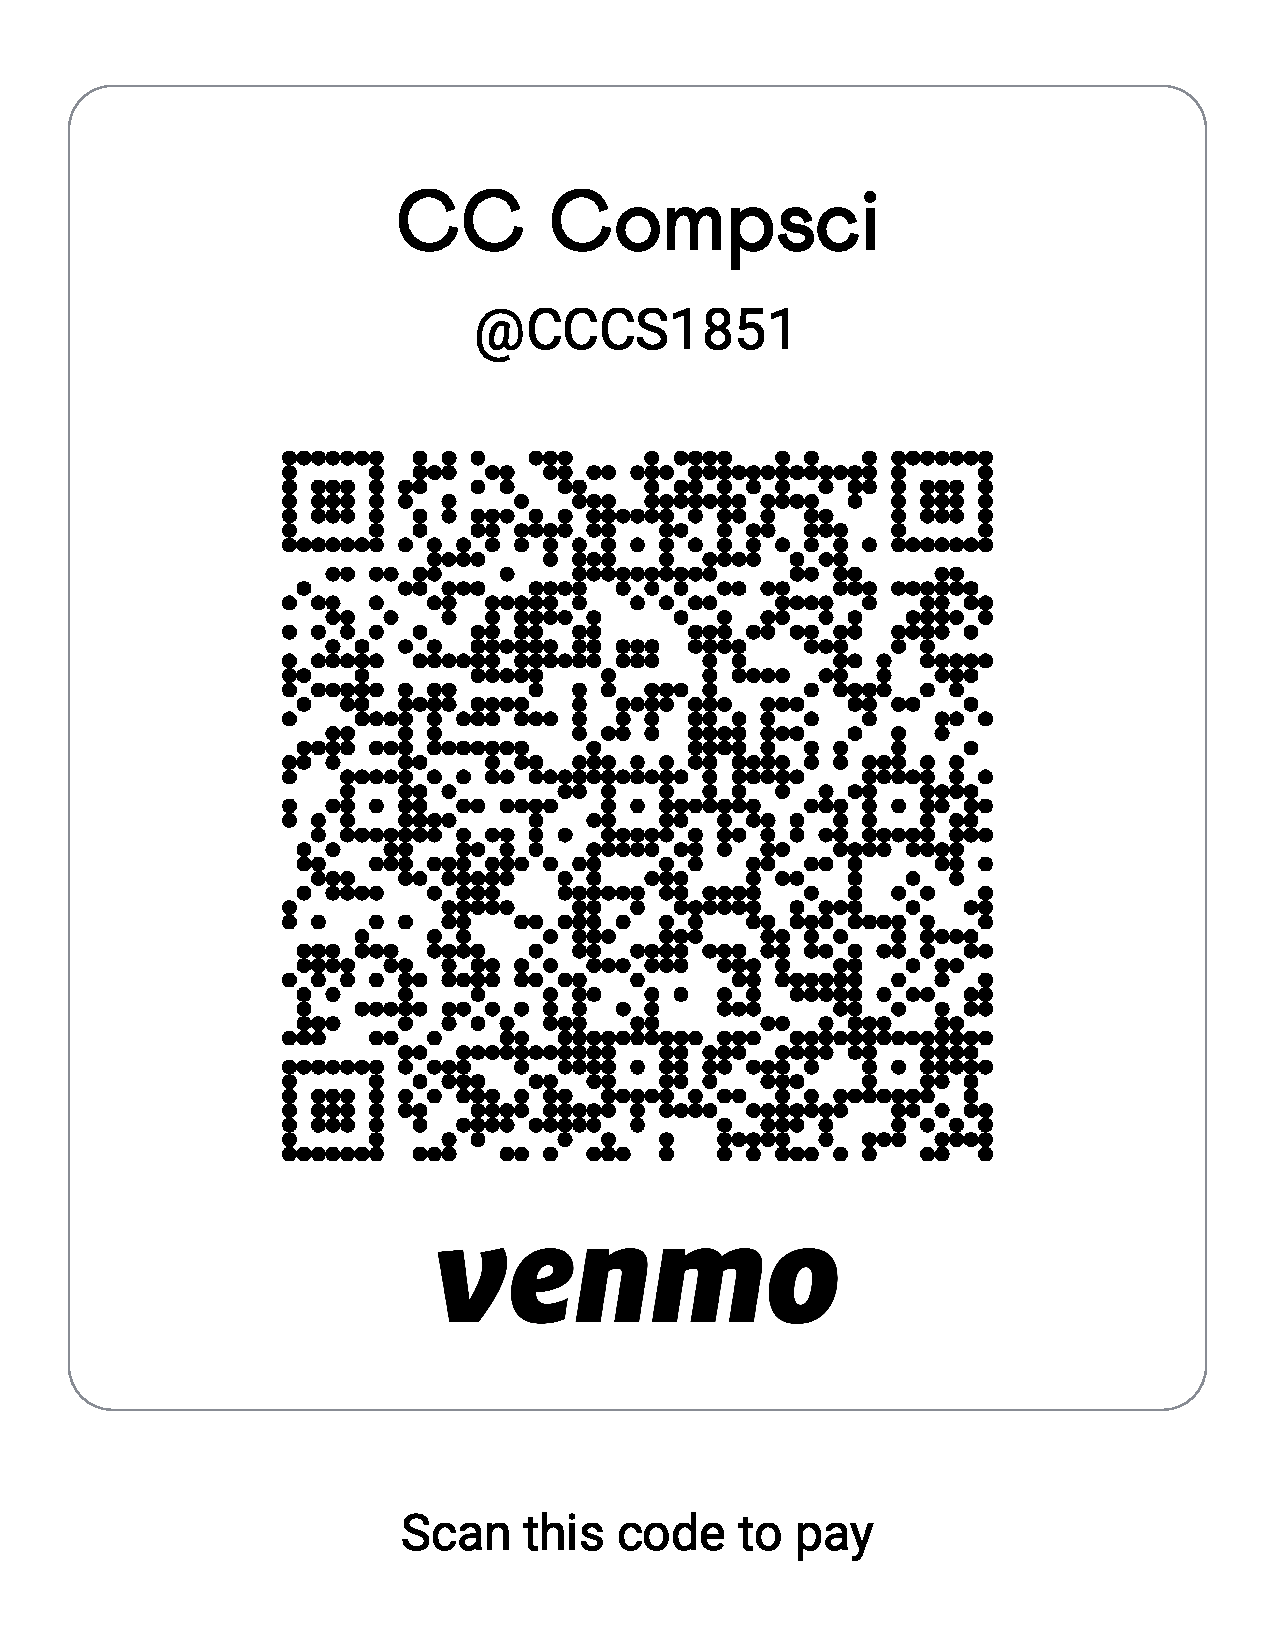
\includegraphics[width=0.9\linewidth]{venmo_qrcode.pdf} % Adjust image width
\end{wrapfigure}
Note that we have support from Columbia College for 100 participants. We want the event to be a success and a valuable experience for as many high school students as possible. Therefore we want a large turnout.
If you change your mind, please inform us ASAP to cancel your registration
so that other high school students can attend the event.

You can request for a full refund by emailing us.
The deadline for request of refund is 5PM, 1/31/2026.

From:
\\
CCCS HS Programming Contest

\end{document}
